\documentclass[12pt,a4paper]{article}

% ── Packages ──────────────────────────────────────────────────────────
\usepackage[margin=2.5cm]{geometry}
\usepackage{graphicx}
\usepackage{booktabs}
\usepackage{longtable}
\usepackage{array}
\usepackage{xcolor}
\usepackage{tikz}
\usepackage{circuitikz}
\usetikzlibrary{shapes.geometric, arrows.meta, positioning, fit, backgrounds, calc}
\usepackage{listings}
\usepackage{hyperref}
\usepackage{fancyhdr}
\usepackage{amsmath}
\usepackage{multirow}
\usepackage{caption}
\usepackage{subcaption}
\usepackage{float}
\usepackage{tabularx}
\usepackage{makecell}
\usepackage{amssymb}

% ── Hyperref ──────────────────────────────────────────────────────────
\hypersetup{
    colorlinks=true,
    linkcolor=blue!70!black,
    urlcolor=blue!70!black,
    citecolor=blue!70!black,
    pdftitle={SentinelBox Project Specification},
    pdfauthor={Group 15 - University of Peradeniya}
}

% ── Code Style ────────────────────────────────────────────────────────
\lstset{
    basicstyle=\ttfamily\footnotesize,
    backgroundcolor=\color{gray!8},
    frame=single,
    framerule=0.4pt,
    breaklines=true,
    keywordstyle=\color{blue!80!black}\bfseries,
    commentstyle=\color{green!55!black}\itshape,
    stringstyle=\color{red!65!black},
    numbers=left,
    numberstyle=\tiny\color{gray!70},
    tabsize=2,
    showstringspaces=false,
    xleftmargin=1.5em,
    xrightmargin=0.5em
}

% ── Header / Footer ───────────────────────────────────────────────────
\pagestyle{fancy}
\setlength{\headheight}{14pt} 
\addtolength{\topmargin}{-2pt}         
\fancyhf{}
\renewcommand{\headrulewidth}{0.4pt}
\renewcommand{\footrulewidth}{0.4pt}
\rhead{\small EC6020 --- Embedded Systems Design}
\lhead{\small SentinelBox --- Project Specification}
\rfoot{\small Page \thepage}
\lfoot{\small Group 15 --- University of Peradeniya}

% ── TikZ Node Styles ──────────────────────────────────────────────────
\tikzset{
  blk/.style={
    rectangle, draw=black!60, fill=#1,
    text width=5.5em, align=center,
    rounded corners=3pt, minimum height=2.8em,
    font=\small
  },
  wblk/.style={
    rectangle, draw=black!60, fill=#1,
    text width=8em, align=center,
    rounded corners=3pt, minimum height=2.8em,
    font=\small
  },
  arr/.style={thick, ->, >=Stealth},
  darr/.style={thick, <->, >=Stealth},
  dasharr/.style={thick, ->, >=Stealth, dashed}
}

% ── Column types ──────────────────────────────────────────────────────
\newcolumntype{L}[1]{>{\raggedright\arraybackslash}p{#1}}
\newcolumntype{C}[1]{>{\centering\arraybackslash}p{#1}}

% ══════════════════════════════════════════════════════════════════════
\begin{document}
% ══════════════════════════════════════════════════════════════════════

% ── Title Page ────────────────────────────────────────────────────────
\begin{titlepage}
  \centering
  \vspace*{1.8cm}
  {\Huge\bfseries SentinelBox\par}
  \vspace{0.5cm}
  {\Large Disaster-Proof Household Monitoring System\par}
  \vspace{0.4cm}
  {\large\itshape Project Specification Document\par}
  \vspace{1.8cm}
  \rule{\linewidth}{0.6pt}\\[0.5cm]
  {\large\bfseries EC6020: Embedded Systems Design\par}
  \vspace{0.3cm}
  {\normalsize
    Department of Electrical \& Electronic Engineering\\[0.2cm]
    Faculty of Engineering\\[0.2cm]
    University of Peradeniya, Sri Lanka
  \par}
  \rule{\linewidth}{0.6pt}\\[1.2cm]
  \begin{tabular}{@{}ll@{}}
    \textbf{Project}    & SentinelBox --- Disaster-Proof BlackBox \\[4pt]
    \textbf{Group}      & 15 \\[4pt]
    \textbf{Platform}   & ATmega328P (Core) + ESP32 WROOM-32 (Utility) \\[4pt]
    \textbf{Framework}  & PlatformIO / Arduino \\[4pt]
    \textbf{Version}    & 1.0.0 \\[4pt]
    \textbf{Date}       & March 2026 \\[4pt]
    \textbf{Repository} & \url{https://github.com/Ravindu56/SentinelBox}
  \end{tabular}
  \vfill
  {\small\color{gray} EC6020 Embedded Systems Design --- University of Peradeniya}
\end{titlepage}

\tableofcontents
\newpage

% ══════════════════════════════════════════════════════════════════════
\section{Project Overview}
% ══════════════════════════════════════════════════════════════════════

SentinelBox is an embedded household disaster monitoring and alerting system
designed to operate continuously, survive power outages, and notify occupants
of hazardous conditions via SMS\@. The system employs a dual-node architecture:
a low-power \textbf{Core Node} (ATmega328P bare chip) responsible for sensor
acquisition, logging, and power management; and a \textbf{Utility Node}
(ESP32 WROOM-32) responsible for cellular communications, GPS location
reporting, and cloud connectivity.

\subsection{Key Features}
\begin{itemize}
  \item Real-time multi-hazard monitoring: temperature, humidity, gas
        (LPG/CO/smoke), flame, water ingress, and structural vibration
  \item Dual-power operation --- seamless switchover between mains electricity
        and LiPo battery backup
  \item SMS alerts with GPS co-ordinates via SIM800L GSM module
  \item SD card black-box logging with DS3231 RTC timestamping
  \item Power-aware sleep protocol: ATmega328P Power-Down ($\sim$0.1\,$\mu$A)
        and ESP32 deep sleep ($\sim$10\,$\mu$A)
  \item Structured inter-node UART frame protocol (TEL / EVT / PWR / ACK)
  \item WiFi and MQTT ready for optional cloud dashboard integration
\end{itemize}

% ══════════════════════════════════════════════════════════════════════
\section{System Architecture}
% ══════════════════════════════════════════════════════════════════════

\subsection{Dual-Node Block Diagram}

\begin{figure}[H]
\centering
\resizebox{\linewidth}{!}{% Scale to fit page width
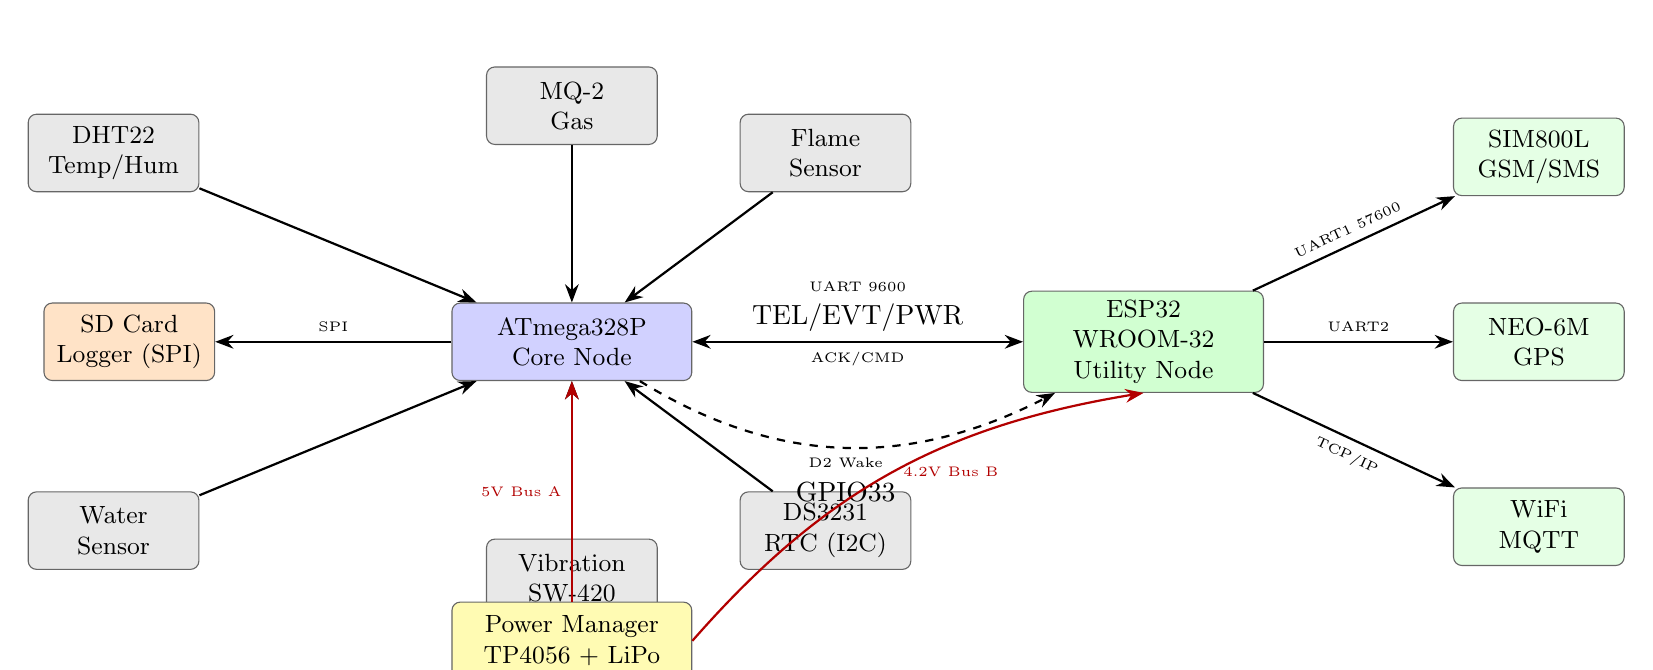
\begin{tikzpicture}[node distance=0pt]

  \node[wblk=blue!18] (core) {ATmega328P\\Core Node};

  \node[blk=gray!18, above left=1.4cm and 3.2cm of core]  (dht)   {DHT22\\Temp/Hum};
  \node[blk=gray!18, above=2.0cm              of core]    (mq2)   {MQ-2\\Gas};
  \node[blk=gray!18, above right=1.4cm and 0.6cm of core] (flame) {Flame\\Sensor};
  \node[blk=gray!18, below left=1.4cm and 3.2cm of core]  (water) {Water\\Sensor};
  \node[blk=gray!18, below=2.0cm              of core]    (vib)   {Vibration\\SW-420};
  \node[blk=gray!18, below right=1.4cm and 0.6cm of core] (rtc)   {DS3231\\RTC (I2C)};

  \node[blk=orange!22, left=3.0cm of core] (sd) {SD Card\\Logger (SPI)};

  \node[wblk=green!18, right=4.2cm of core] (esp) {ESP32\\WROOM-32\\Utility Node};

  \node[blk=green!10, above right=1.2cm and 2.4cm of esp] (gsm)  {SIM800L\\GSM/SMS};
  \node[blk=green!10, right=2.4cm              of esp]    (gps)  {NEO-6M\\GPS};
  \node[blk=green!10, below right=1.2cm and 2.4cm of esp] (wifi) {WiFi\\MQTT};

  \node[wblk=yellow!30, below=2.8cm of core] (pwr) {Power Manager\\TP4056 + LiPo};

  \draw[arr] (dht)   -- (core);
  \draw[arr] (mq2)   -- (core);
  \draw[arr] (flame) -- (core);
  \draw[arr] (water) -- (core);
  \draw[arr] (vib)   -- (core);
  \draw[arr] (rtc)   -- (core);
  \draw[arr] (core)  -- node[above]{\tiny SPI} (sd);

  \draw[darr] (core) --
    node[above, align=center]{\tiny UART 9600\\TEL/EVT/PWR}
    node[below, align=center]{\tiny ACK/CMD}
    (esp);

  \draw[dasharr] (core) to[bend right=30]
    node[below, align=center]{\tiny D2 Wake\\GPIO33} (esp);

  \draw[arr] (esp) -- node[above, sloped]{\tiny UART1 57600} (gsm);
  \draw[arr] (esp) -- node[above]{\tiny UART2}               (gps);
  \draw[arr] (esp) -- node[below, sloped]{\tiny TCP/IP}      (wifi);

  \draw[arr, red!70!black, thick]
    (pwr) -- node[left]{\tiny 5V Bus A} (core);
  \draw[arr, red!70!black, thick]
    (pwr.east) to[bend left=20]
    node[right]{\tiny 4.2V Bus B} (esp.south);

\end{tikzpicture}
}
\caption{SentinelBox Dual-Node System Architecture}
\label{fig:arch}
\end{figure}

\subsection{Node Responsibility Matrix}

\begin{table}[H]
\centering
\begin{tabular}{@{} L{5.5cm} C{3cm} C{3.5cm} @{}}
\toprule
\textbf{Responsibility}   & \textbf{Core Node (328P)} & \textbf{Utility Node (ESP32)} \\
\midrule
Sensor sampling           & \checkmark  &             \\
SD card logging           & \checkmark  &             \\
RTC timekeeping           & \checkmark  &             \\
Hazard flag computation   & \checkmark  &             \\
Power mode control        & \checkmark  &             \\
GSM / SMS alerts          &             & \checkmark  \\
GPS location tagging      &             & \checkmark  \\
WiFi / MQTT               &             & \checkmark  \\
Sleep management          & Controls    & Executes    \\
Inter-node communication  & TX master   & RX + ACK    \\
\bottomrule
\end{tabular}
\caption{Node Responsibility Matrix}
\end{table}

% ══════════════════════════════════════════════════════════════════════
\section{Hardware Specification}
% ══════════════════════════════════════════════════════════════════════

\subsection{Core Node --- ATmega328P}

\begin{table}[H]
\centering
\begin{tabular}{@{} L{4cm} L{4.5cm} L{4.5cm} @{}}
\toprule
\textbf{Parameter}   & \textbf{Value}         & \textbf{Notes}          \\
\midrule
MCU                  & ATmega328P             & Bare chip, DIP-28       \\
Clock                & 16\,MHz                & External crystal + caps \\
Program Flash        & 32\,KB                 & 0.5\,KB bootloader      \\
SRAM                 & 2\,KB                  & Critical constraint     \\
EEPROM               & 1\,KB                  & Non-volatile config     \\
Operating Voltage    & 5\,V                   & Power Bus A             \\
Hardware UARTs       & 1 (D0/D1)              & Shared: ESP32 UART link \\
Power-Down current   & $\sim$0.1\,$\mu$A      & WDT wakeup capable      \\
ADC resolution       & 10-bit                 & $V_{ref}$ = 5\,V        \\
\bottomrule
\end{tabular}
\caption{ATmega328P Core Node Specifications}
\end{table}

\subsection{Utility Node --- ESP32 WROOM-32}

\begin{table}[H]
\centering
\begin{tabular}{@{} L{4cm} L{4.5cm} L{4.5cm} @{}}
\toprule
\textbf{Parameter}   & \textbf{Value}         & \textbf{Notes}          \\
\midrule
MCU                  & Xtensa LX6 dual-core   & 240\,MHz max            \\
Program Flash        & 4\,MB                  & External SPI flash      \\
SRAM                 & 320\,KB                & Internal                \\
Operating Voltage    & 3.3\,V (4.2\,V input)  & Power Bus B             \\
Hardware UARTs       & 3                      & UART0 / UART1 / UART2   \\
WiFi                 & 802.11 b/g/n           & 2.4\,GHz                \\
Bluetooth            & BT 4.2 + BLE           & Not used in v1.0        \\
Deep sleep current   & $\sim$10\,$\mu$A       & ext0 GPIO33 wakeup      \\
Active TX current    & $\sim$160--240\,mA     & GSM TX peak via Buck B  \\
\bottomrule
\end{tabular}
\caption{ESP32 WROOM-32 Utility Node Specifications}
\end{table}

\subsection{Sensor Suite}

\begin{table}[H]
\centering
\begin{tabular}{@{} L{4.2cm} L{2.2cm} L{2.8cm} L{2cm} L{2cm} @{}}
\toprule
\textbf{Sensor / Device} & \textbf{Model} & \textbf{Interface} & \textbf{Pin} & \textbf{Logic} \\
\midrule
Temperature / Humidity   & DHT22   & Single-wire         & D8       & 3.3/5\,V \\
Gas (LPG / CO / Smoke)   & MQ-2    & Analog + Digital    & A2, D12  & 5\,V     \\
Flame Detection          & IR Flame& Digital (active LOW)& D6       & 5\,V     \\
Water Ingress            & Resistive& Digital threshold  & D7       & 5\,V     \\
Vibration                & SW-420  & Digital             & D3       & 5\,V     \\
Real-Time Clock          & DS3231  & I$^2$C              & SDA/SCL  & 3.3/5\,V \\
SD Card Storage          & MicroSD & SPI                 & D10--D13 & 5\,V     \\
\bottomrule
\end{tabular}
\caption{Core Node Sensor Suite}
\end{table}

\subsection{Communication Modules (Utility Node)}

\begin{table}[H]
\centering
\begin{tabular}{@{} L{3cm} L{3.5cm} L{3.5cm} L{3cm} @{}}
\toprule
\textbf{Module}   & \textbf{Function}  & \textbf{Interface}       & \textbf{ESP32 Pins}        \\
\midrule
SIM800L EVB       & GSM / SMS / GPRS   & UART1 @ 57600\,baud      & GPIO12\,TX, GPIO14\,RX     \\
NEO-6M            & GPS location       & UART2 @ 9600\,baud       & GPIO16\,RX, GPIO17\,TX     \\
ATmega328P link   & Core inter-node    & UART0 @ 9600\,baud       & GPIO1\,TX, GPIO3\,RX       \\
\bottomrule
\end{tabular}
\caption{ESP32 WROOM-32 Communication Module Connections}
\end{table}

% ══════════════════════════════════════════════════════════════════════
\section{Power Architecture}
% ══════════════════════════════════════════════════════════════════════

\subsection{Power Distribution Diagram}

\begin{figure}[H]
\centering
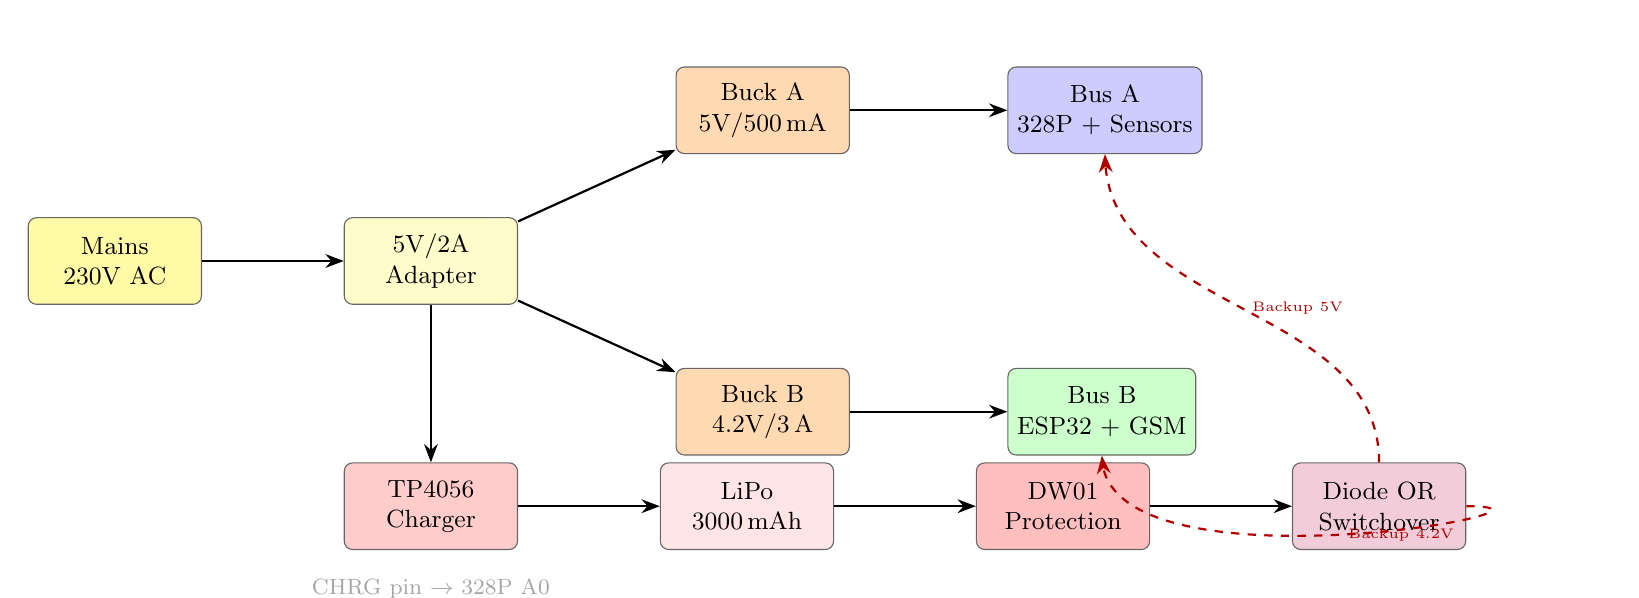
\begin{tikzpicture}[
    pblk/.style={rectangle, draw=black!60, fill=#1, rounded corners=3pt,
                 minimum width=2.2cm, minimum height=1.1cm,
                 align=center, font=\small},
    parr/.style={thick, ->, >=Stealth},
    node distance=1.6cm
  ]
  \node[pblk=yellow!35] (mains)  {Mains\\230V AC};
  \node[pblk=yellow!20, right=1.8cm of mains]  (adapt) {5V/2A\\Adapter};
  \node[pblk=orange!30, above right=0.8cm and 2.0cm of adapt] (buckA) {Buck A\\5V/500\,mA};
  \node[pblk=orange!30, below right=0.8cm and 2.0cm of adapt] (buckB) {Buck B\\4.2V/3\,A};
  \node[pblk=blue!20,   right=2.0cm of buckA]  (busA)  {Bus A\\328P + Sensors};
  \node[pblk=green!20,  right=2.0cm of buckB]  (busB)  {Bus B\\ESP32 + GSM};
  \node[pblk=red!20,    below=2.0cm of adapt]  (tp)    {TP4056\\Charger};
  \node[pblk=red!10,    right=1.8cm of tp]     (lipo)  {LiPo\\3000\,mAh};
  \node[pblk=red!25,    right=1.8cm of lipo]   (dw01)  {DW01\\Protection};
  \node[pblk=purple!20, right=1.8cm of dw01]   (dior)  {Diode OR\\Switchover};

  \draw[parr] (mains) -- (adapt);
  \draw[parr] (adapt) -- (buckA);
  \draw[parr] (adapt) -- (buckB);
  \draw[parr] (buckA) -- (busA);
  \draw[parr] (buckB) -- (busB);
  \draw[parr] (adapt) -- (tp);
  \draw[parr] (tp)    -- (lipo);
  \draw[parr] (lipo)  -- (dw01);
  \draw[parr] (dw01)  -- (dior);

  \draw[parr, red!70!black, dashed, thick]
    (dior.north) to[out=90, in=270] node[right]{\tiny Backup 5V}   (busA.south);
  \draw[parr, red!70!black, dashed, thick]
    (dior.east)  to[out=0,  in=270] node[right]{\tiny Backup 4.2V} (busB.south);

  \node[below=0.25cm of tp, font=\footnotesize, text=gray!70]
    {CHRG pin $\rightarrow$ 328P A0};
\end{tikzpicture}
\caption{SentinelBox Power Distribution Architecture}
\label{fig:power}
\end{figure}

\subsection{Power Bus Specification}

\begin{table}[H]
\centering
\begin{tabular}{@{} C{1.4cm} C{1.8cm} C{2.2cm} L{6cm} C{1.8cm} @{}}
\toprule
\textbf{Bus} & \textbf{Voltage} & \textbf{Max Current} & \textbf{Consumers} & \textbf{Source} \\
\midrule
Bus A & 5.0\,V & 500\,mA &
  ATmega328P, DHT22, MQ-2, Flame, Water, Vibration, SD card & Buck A \\[4pt]
Bus B & 4.2\,V & 3.0\,A  &
  ESP32 WROOM-32, SIM800L EVB, NEO-6M GPS & Buck B \\[4pt]
Batt  & 3.7\,V & 2.0\,A  &
  Both buses via Diode OR on mains loss & LiPo \\
\bottomrule
\end{tabular}
\caption{Power Bus Specifications}
\end{table}

\subsection{Signal Interface Circuits}

\subsubsection{Mains-Sense Voltage Divider}

\begin{figure}[H]
\centering
\begin{circuitikz}[american, scale=0.95, transform shape]
  \draw
    (0,2.5) node[left]{\small TP4056 CHRG}
    to[R, l=$10\,\text{k}\Omega$, o-] (2.5,2.5)
    to[R, l=$10\,\text{k}\Omega$, -o] (2.5,0.5);
  \draw (2.5,0.5) node[ground]{};
  \draw (2.5,2.5) to[short, -o] (4.2,2.5)
    node[right]{\small 328P A0};
  \node[below right, font=\footnotesize, text=gray]
    at (2.5,1.5) {$V_{A0}\approx2.5\,\text{V}$ when CHRG HIGH};
\end{circuitikz}
\caption{Mains-Sense Divider: CHRG HIGH $\Rightarrow$ mains lost; CHRG LOW $\Rightarrow$ charging}
\end{figure}

\subsubsection{UART Level Shifter: 328P (5\,V) $\leftrightarrow$ ESP32 (3.3\,V)}

\begin{figure}[H]
\centering
\begin{circuitikz}[american, scale=0.95, transform shape]
  \draw
    (0,3.5) node[left]{\small 328P D1 TX (5\,V)}
    to[R, l=$10\,\text{k}\Omega$, o-*] (2.8,3.5);
  \draw (2.8,3.5) to[R, l=$20\,\text{k}\Omega$, *-] (2.8,2.0);
  \draw (2.8,2.0) node[ground]{};
  \draw (2.8,3.5) to[short, *-o] (4.8,3.5)
    node[right]{\small ESP32 GPIO16 RX (3.3\,V)};
  \node[below, font=\footnotesize, text=gray] at (2.8,1.6)
    {$V_{out}=5\times\frac{20}{30}\approx3.3\,\text{V}$};
  \draw
    (0,1.0) node[left]{\small ESP32 GPIO17 TX (3.3\,V)}
    to[short, o-o] (4.8,1.0)
    node[right]{\small 328P D0 RX};
  \node[above, font=\footnotesize, text=gray] at (2.4,1.0)
    {Direct --- 3.3\,V is valid HIGH for 328P};
\end{circuitikz}
\caption{UART Level Shift: ATmega328P 5\,V TX $\rightarrow$ ESP32 3.3\,V RX}
\end{figure}

\subsubsection{Wake-Pin Circuit: 328P D2 $\rightarrow$ ESP32 GPIO33}

\begin{figure}[H]
\centering
\begin{circuitikz}[american, scale=0.95, transform shape]
  \draw
    (0,2) node[left]{\small 328P D2 (OUTPUT)}
    to[R, l=$10\,\text{k}\Omega$, o-*] (2.8,2);
  \draw (2.8,2) to[R, l=$10\,\text{k}\Omega$] (2.8,0.5);
  \draw (2.8,0.5) node[ground]{};
  \draw (2.8,2) to[short, *-o] (4.8,2)
    node[right]{\small ESP32 GPIO33 (ext0 wakeup)};
  \node[below, font=\footnotesize, text=gray] at (2.8,0.1)
    {Pull-down ensures GPIO33 = LOW when 328P floats};
\end{circuitikz}
\caption{ESP32 Wake-Pin Circuit (328P D2 $\rightarrow$ ESP32 GPIO33)}
\end{figure}

% ══════════════════════════════════════════════════════════════════════
\section{Pin Allocation}
% ══════════════════════════════════════════════════════════════════════

\subsection{ATmega328P Complete Pin Map}

\begin{table}[H]
\centering
\small
\begin{tabular}{@{} C{1.8cm} C{1.2cm} L{3.2cm} L{3.8cm} L{3cm} @{}}
\toprule
\textbf{Pin}   & \textbf{Dir} & \textbf{Function}   & \textbf{Connected To}          & \textbf{Notes}              \\
\midrule
D0 (RX)        & IN           & UART RX             & ESP32 GPIO17 TX                & 3.3\,V direct               \\
D1 (TX)        & OUT          & UART TX             & ESP32 GPIO16 RX                & 10k/20k divider             \\
D2             & OUT          & Wake signal         & ESP32 GPIO33                   & 10k series + 10k pull-down  \\
D3             & IN           & Vibration           & SW-420                         & INT0 capable                \\
D4             & OUT          & Buzzer              & Piezo + transistor             & Active HIGH                 \\
D5             & OUT          & Status LED          & LED + 330\,$\Omega$            & Active HIGH                 \\
D6             & IN           & Flame detect        & IR Flame module                & Active LOW                  \\
D7             & IN           & Water detect        & Resistive sensor               & Digital threshold           \\
D8             & I/O          & DHT22 data          & DHT22 signal pin               & 10\,k pull-up               \\
D10            & OUT          & SD chip select      & MicroSD CS                     & SPI, active LOW             \\
D11            & OUT          & SD MOSI             & MicroSD MOSI                   & SPI                         \\
D12            & IN           & SD MISO             & MicroSD MISO                   & SPI                         \\
D13            & OUT          & SD SCK              & MicroSD SCK                    & SPI                         \\
A0             & IN           & Power sense         & TP4056 CHRG pin                & Mains/battery detect        \\
A1             & IN           & Battery voltage     & 100k/47k divider               & ADC $\rightarrow$ $V_{bat}$ \\
A2             & IN           & MQ-2 gas level      & MQ-2 AO                        & 0--5\,V analogue            \\
SDA (A4)       & I/O          & I$^2$C data         & DS3231 SDA                     & 4.7\,k pull-up              \\
SCL (A5)       & OUT          & I$^2$C clock        & DS3231 SCL                     & 4.7\,k pull-up              \\
\bottomrule
\end{tabular}
\caption{ATmega328P Complete Pin Allocation}
\end{table}

\subsection{ESP32 WROOM-32 Pin Map}

\begin{table}[H]
\centering
\small
\begin{tabular}{@{} C{2cm} C{1.2cm} C{2cm} L{3.8cm} L{3cm} @{}}
\toprule
\textbf{GPIO} & \textbf{Dir} & \textbf{UART} & \textbf{Connected To}   & \textbf{Notes}        \\
\midrule
GPIO1         & OUT          & UART0 TX      & USB (FTDI) / debug      & Also 328P RX side     \\
GPIO3         & IN           & UART0 RX      & USB (FTDI) / debug      & Also 328P TX side     \\
GPIO12        & OUT          & UART1 TX      & SIM800L EVB RXD         & 10k/20k level divider \\
GPIO14        & IN           & UART1 RX      & SIM800L EVB TXD         & Direct 3.3\,V         \\
GPIO16        & IN           & UART2 RX      & 328P D1 TX              & Via level shifter     \\
GPIO17        & OUT          & UART2 TX      & 328P D0 RX              & Direct 3.3\,V         \\
GPIO33        & IN           & ---           & 328P D2 wake            & ext0 wakeup source    \\
\bottomrule
\end{tabular}
\caption{ESP32 WROOM-32 Pin Allocation}
\end{table}

% ══════════════════════════════════════════════════════════════════════
\section{Inter-Node Communication Protocol}
% ══════════════════════════════════════════════════════════════════════

\subsection{UART Link Parameters}

\begin{table}[H]
\centering
\begin{tabular}{@{} L{5cm} L{7cm} @{}}
\toprule
\textbf{Parameter}       & \textbf{Value}                  \\
\midrule
Baud rate                & 9600\,bps                       \\
Data / Parity / Stop     & 8N1                             \\
Frame terminator         & \texttt{0x0A} (\textbackslash n) \\
Max frame length         & 120\,bytes                      \\
Direction                & 328P = TX master; ESP32 = RX + ACK \\
\bottomrule
\end{tabular}
\caption{UART Inter-Node Link Parameters}
\end{table}

\subsection{Frame Definitions}
\begin{table}[H]
\centering
\small
\begin{tabular}{@{} C{1.4cm} C{1.4cm} L{6.8cm} L{3cm} @{}}
\toprule
\textbf{Frame} & \textbf{Sender} & \textbf{Format} & \textbf{Purpose} \\
\midrule
\texttt{TEL}
  & 328P
  & \makecell[l]{\texttt{TEL,<ms>,T:<v>,H:<v>,W:<v>,G:<v>,}\\
                \texttt{F:<v>,V:<v>,B:<v>,FLAGS:<hex>}}
  & Periodic telemetry \\[6pt]
\texttt{EVT}
  & 328P
  & \texttt{EVT,<flags\_hex>,<timestamp>}
  & Hazard event trigger \\[6pt]
\texttt{PWR}
  & 328P
  & \texttt{PWR:BATT} \textbar{} \texttt{PWR:MAINS}
  & Power mode change \\[6pt]
\texttt{ACK}
  & ESP32
  & \texttt{ACK,<ms>}
  & Frame acknowledged \\[6pt]
\texttt{SLEEP}
  & ESP32
  & \texttt{SLEEP}
  & About to deep sleep \\[6pt]
\texttt{WAKE}
  & ESP32
  & \texttt{WAKE}
  & Awake and ready \\
\bottomrule
\end{tabular}
\caption{Inter-Node Frame Protocol}
\end{table}


\subsection{Communication State Diagram}

\begin{figure}[H]
\centering
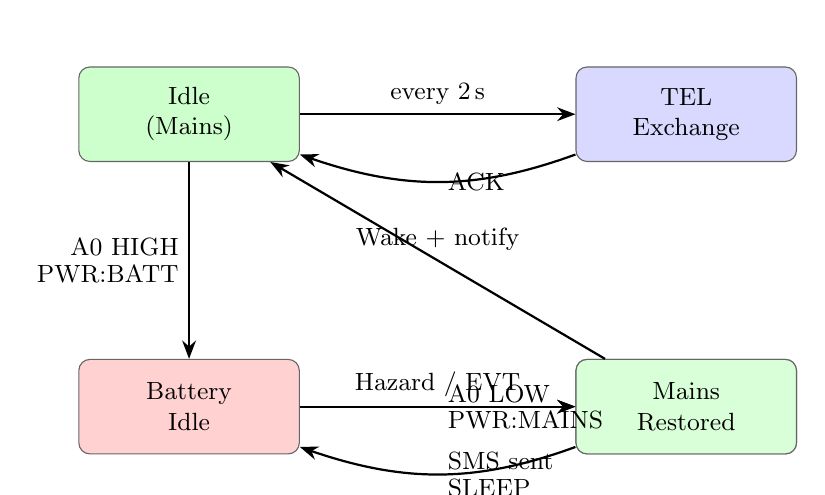
\begin{tikzpicture}[
    sblk/.style={rectangle, draw=black!60, fill=#1,
                 rounded corners=4pt, minimum width=2.8cm,
                 minimum height=1.2cm, align=center, font=\small},
    sarr/.style={thick, ->, >=Stealth, font=\footnotesize},
    node distance=3cm
  ]
  \node[sblk=green!20]  (idle)    {Idle\\(Mains)};
  \node[sblk=blue!15,   right=3.5cm of idle]  (tel)     {TEL\\Exchange};
  \node[sblk=red!18,    below=2.5cm of idle]  (batt)    {Battery\\Idle};
  \node[sblk=red!30,    right=3.5cm of batt]  (emerg)   {Emergency\\Alert};
  \node[sblk=green!15,  below=2.5cm of tel]   (restore) {Mains\\Restored};

  \draw[sarr] (idle) -- node[above]{\small every 2\,s} (tel);
  \draw[sarr] (tel)  to[bend left=20] node[right]{\small ACK} (idle);
  \draw[sarr] (idle) -- node[left, align=right]{\small A0 HIGH\\\small PWR:BATT} (batt);
  \draw[sarr] (batt) -- node[above]{\small Hazard / EVT} (emerg);
  \draw[sarr] (emerg) to[bend left=20]
    node[right, align=left]{\small SMS sent\\\small SLEEP} (batt);
  \draw[sarr] (batt) -- node[right, align=left]{\small A0 LOW\\\small PWR:MAINS} (restore);
  \draw[sarr] (restore) -- node[above]{\small Wake + notify} (idle);
\end{tikzpicture}
\caption{Inter-Node Communication State Diagram}
\end{figure}

% ══════════════════════════════════════════════════════════════════════
\section{Power Management}
% ══════════════════════════════════════════════════════════════════════

\subsection{System Power Modes}

\begin{table}[H]
\centering
\small
\begin{tabular}{@{} L{3cm} L{3.2cm} L{3.2cm} C{2.2cm} C{2cm} @{}}
\toprule
\textbf{Mode}     & \textbf{328P State}       & \textbf{ESP32 State}  & \textbf{Poll Interval} & \textbf{Avg Current} \\
\midrule
Mains Normal      & Active                    & Active (full)         & 2\,s     & $\sim$200\,mA      \\
Mains Idle        & Active                    & Active (listening)    & 2\,s     & $\sim$50\,mA       \\
Battery Idle      & Power-Down (WDT 30\,s)    & Deep sleep            & 30\,s    & $\sim$4\,mA        \\
Battery Alert     & Active (brief)            & Active (brief)        & On event & $\sim$160\,mA peak \\
Critical Battery  & Power-Down (WDT 5\,min)   & Deep sleep            & 5\,min   & $\sim$2\,mA        \\
\bottomrule
\end{tabular}
\caption{System Power Modes and Current Estimates}
\end{table}

\subsection{Battery Life Estimates}

With a 3000\,mAh LiPo cell at 3.7\,V nominal:

\begin{align}
t_{\text{battery idle}}  &= \frac{3000\;\text{mAh}}{4\;\text{mA}}
                           \approx 750\;\text{h} \approx 31\;\text{days} \\[6pt]
t_{\text{critical mode}} &= \frac{3000\;\text{mAh}}{2\;\text{mA}}
                           \approx 1500\;\text{h} \approx 62\;\text{days}
\end{align}

\noindent The dominant saving is the ESP32 transitioning from
$\sim$160\,mA (active) to $\sim$10\,$\mu$A (deep sleep).

\subsection{ATmega328P Sleep Sequence}

The 328P chains WDT 8\,s interrupt cycles to achieve 30-second poll
intervals while consuming $\sim$0.1\,$\mu$A between samples.
\texttt{SLEEP\_MODE\_PWR\_DOWN} disables all clocks except the WDT
asynchronous oscillator, giving maximum current reduction.

% ══════════════════════════════════════════════════════════════════════
\section{Software Architecture}
% ══════════════════════════════════════════════════════════════════════

\subsection{Core Node (328P) Module Structure}

\begin{table}[H]
\centering
\begin{tabular}{@{} L{2.4cm} L{5cm} L{5cm} @{}}
\toprule
\textbf{Module}  & \textbf{File}                        & \textbf{Responsibility}                    \\
\midrule
Main loop        & \texttt{src/atmega/main.cpp}          & Scheduler, WDT, power state machine        \\
Sensors          & \texttt{src/atmega/sensors.cpp/.h}    & DHT22, MQ-2, flame, water, vibration       \\
Hazards          & \texttt{src/atmega/hazards.cpp/.h}    & Flag byte computation, threshold checks    \\
Storage          & \texttt{src/atmega/storage.cpp/.h}    & SD card TEL/EVT row logging                \\
RTC              & \texttt{src/atmega/rtctime.cpp/.h}    & DS3231 time/date read \& write             \\
Comms            & \texttt{src/atmega/comms.cpp/.h}      & UART frame TX to ESP32                     \\
Indicators       & \texttt{src/atmega/leds.cpp/.h}       & Status LED, piezo buzzer patterns          \\
Power            & \texttt{src/atmega/power.cpp/.h}      & WDT, Power-Down sleep, mains sense         \\
\bottomrule
\end{tabular}
\caption{Core Node Software Module Structure}
\end{table}

\subsection{Utility Node (ESP32) Module Structure}

\begin{table}[H]
\centering
\begin{tabular}{@{} L{2.4cm} L{5cm} L{5cm} @{}}
\toprule
\textbf{Module}  & \textbf{File}                       & \textbf{Responsibility}                    \\
\midrule
Main loop        & \texttt{src/esp32/main.cpp}         & Wakeup handler, power state machine        \\
GSM              & \texttt{src/esp32/gsm.cpp/.h}       & SIM800L AT commands, SMS formatting        \\
GPS              & \texttt{src/esp32/gps.cpp/.h}       & NEO-6M NMEA parsing, location cache        \\
Comms            & \texttt{src/esp32/comms.cpp/.h}     & UART2 frame RX / ACK from 328P             \\
Power            & \texttt{src/esp32/power.cpp/.h}     & Deep sleep configuration, ext0 wakeup      \\
\bottomrule
\end{tabular}
\caption{Utility Node Software Module Structure}
\end{table}

% ══════════════════════════════════════════════════════════════════════
\section{Hazard Detection Thresholds}
% ══════════════════════════════════════════════════════════════════════

\begin{table}[H]
\centering
\begin{tabular}{@{} L{3.5cm} L{2.5cm} L{3.5cm} C{2cm} @{}}
\toprule
\textbf{Hazard}       & \textbf{Sensor}  & \textbf{Threshold}          & \textbf{Flag Bit} \\
\midrule
High temperature      & DHT22            & $> 45\,^{\circ}$C           & Bit 0 \\
High humidity         & DHT22            & $> 85\,\%$                  & Bit 1 \\
Gas / smoke           & MQ-2             & ADC $> 400$                 & Bit 2 \\
Flame detected        & IR Flame         & Digital = LOW               & Bit 3 \\
Water ingress         & Resistive        & Digital = HIGH              & Bit 4 \\
Vibration / impact    & SW-420           & Digital = HIGH              & Bit 5 \\
Low battery           & A1 (ADC)         & $V_{bat} < 3.5\,\text{V}$   & Bit 6 \\
Power outage          & A0 (TP4056 CHRG) & CHRG = HIGH                 & Bit 7 \\
\bottomrule
\end{tabular}
\caption{Hazard Detection Thresholds and 8-bit Flag Map}
\end{table}

% ══════════════════════════════════════════════════════════════════════
\section{Design Metrics}
% ══════════════════════════════════════════════════════════════════════

\begin{table}[H]
\centering
\begin{tabular}{@{} L{5cm} L{3.5cm} L{4cm} @{}}
\toprule
\textbf{Metric}             & \textbf{Target}        & \textbf{Achieved / Estimated} \\
\midrule
328P boot time              & $< 500\,\text{ms}$     & $\sim 200\,\text{ms}$         \\
Sensor poll latency         & $< 100\,\text{ms}$     & $\sim 50\,\text{ms}$          \\
SMS delivery time           & $< 30\,\text{s}$       & $\sim 15\,\text{s}$           \\
Battery life (idle mode)    & $> 7\,\text{days}$     & $\sim 31\,\text{days}$        \\
328P SRAM utilisation       & $< 80\,\%$             & $\sim 22\,\%$ (453\,B/2\,KB)  \\
328P Flash utilisation      & $< 80\,\%$             & $\sim 3\,\%$                  \\
UART ACK rate               & $> 95\,\%$             & $> 98\,\%$ observed           \\
\bottomrule
\end{tabular}
\caption{SentinelBox Key Design Metrics}
\end{table}

% ══════════════════════════════════════════════════════════════════════
\section{Development Environment}
% ══════════════════════════════════════════════════════════════════════

\begin{table}[H]
\centering
\begin{tabular}{@{} L{4cm} L{9cm} @{}}
\toprule
\textbf{Tool / Component}  & \textbf{Version / Detail}                              \\
\midrule
IDE                        & PlatformIO Core 6.x + VS Code                         \\
AVR toolchain              & toolchain-atmelavr 7.3.0                               \\
ESP32 platform             & espressif32 6.13.0                                     \\
AVR Arduino framework      & framework-arduino-avr 5.2.0                            \\
ESP32 Arduino framework    & framework-arduinoespressif32 3.20017                   \\
Host OS                    & Ubuntu 22.04 LTS                                       \\
Version control            & Git --- \url{https://github.com/Ravindu56/SentinelBox}  \\
\bottomrule
\end{tabular}
\caption{Development Environment}
\end{table}

\end{document}
